\documentclass[xetex,mathsans,sans,aspectratio=169]{beamer}
\usepackage{listings}
\usetheme{Boadilla}
\usecolortheme{orchid}
\usepackage{fontspec}
\setsansfont{Basis Grotesque}
\setbeamertemplate{navigation symbols}{}
\usepackage{amsmath}
\usepackage{multicol}


\title[Building end-to-end encrypted decentralized applications with nucypher]{
\includegraphics[width=5.5cm]{pdf/nucypher_logo.pdf}}
\author[Michael and John]{Michael Egorov and John Pacific}
\date[10 Sep]{Decentralized stack developers meetup, 10 Sep 2018}

\begin{document}
    \begin{frame}
        \titlepage
    \end{frame}

    \begin{frame}
        \frametitle{Central server + TLS}
        \framesubtitle{Data vulnerable to hackers, state actors etc}
        \begin{figure}
            \centering
            \includegraphics[width=11cm]{pdf/file-sharing-tls.pdf}
        \end{figure}
    \end{frame}

    \begin{frame}
        \frametitle{Why}
        \framesubtitle{Encrypted multi-user chats}
        \begin{figure}
            \centering
            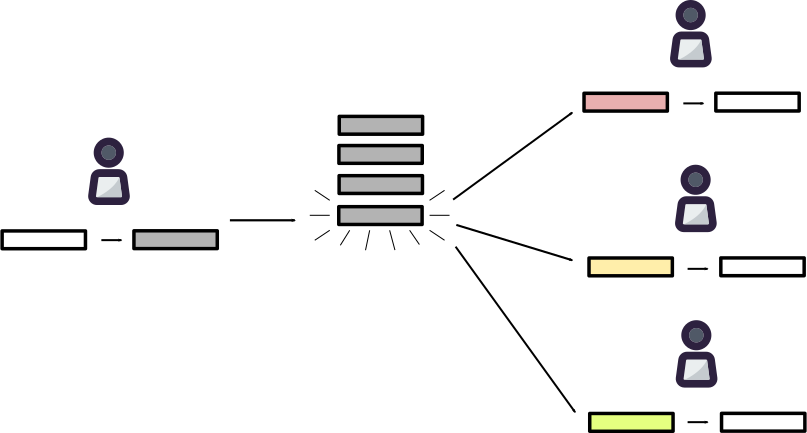
\includegraphics[height=5.5cm]{pdf/chats.pdf}
        \end{figure}
    \end{frame}

    \begin{frame}
        \frametitle{What is proxy re-encryption (PRE)}
        \begin{figure}
            \centering
            \includegraphics[width=11cm]{pdf/pre.pdf}
        \end{figure}
    \end{frame}

    \begin{frame}
        \frametitle{Key management using PRE}
        \framesubtitle{Decryption}
        \begin{figure}
            \centering
            \includegraphics[height=5.5cm]{pdf/decrypt.pdf}
        \end{figure}
    \end{frame}

    \begin{frame}
        \frametitle{Decentralized key management}
        \framesubtitle{Using threshold split-key re-encryption (Umbral)}
        \begin{figure}
            \centering
            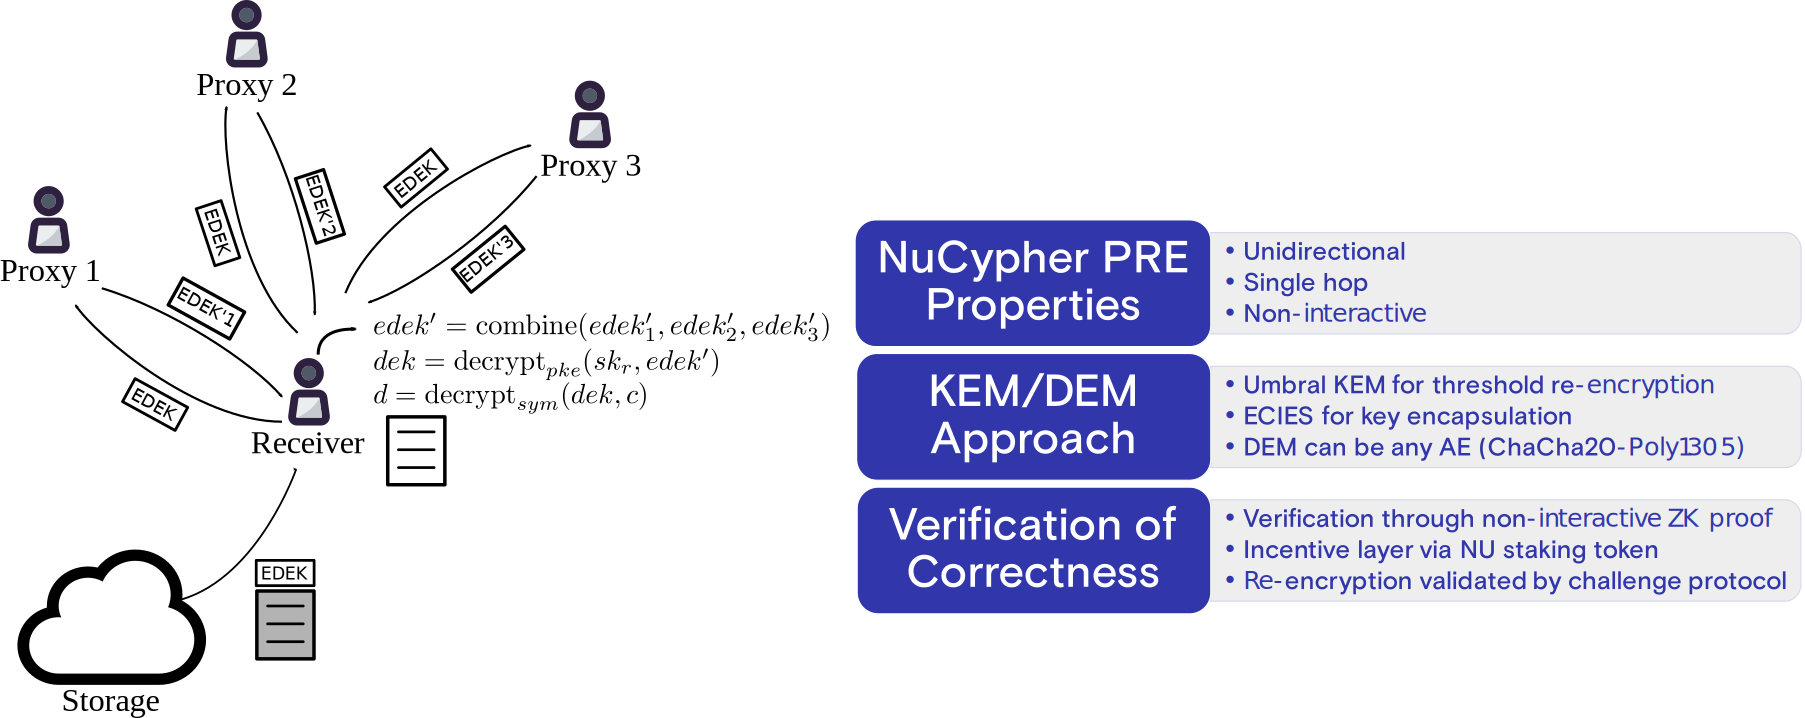
\includegraphics[height=6.5cm]{pdf/decrypt-umbral.pdf}
        \end{figure}
        \url{https://github.com/nucypher/nucypher-kms/}
        \url{https://github.com/nucypher/pyUmbral/}
    \end{frame}


    \begin{frame}
        \frametitle{Umbral: threshold proxy re-encryption}
        %\framesubtitle{Purpose}
        \begin{itemize}
        	\item \emph{``Umbral''} is Spanish for \emph{``threshold''}
            \item PRE properties: Unidirectional, single-hop, non-interactive
            \item It follows a KEM/DEM approach:
            	\begin{itemize}
					\item UmbralKEM provides the threshold re-encryption capability
                    \item Uses ECIES for key encapsulation with zero knowledge proofs of correctness for verifiability on prime order curves (such as secp256k1)
            		\item The DEM can be any authenticated encryption (currently ChaCha20-Poly1305)
        		\end{itemize}
			\item IND-PRE-CCA security
			\item Verification of re-encryption correctness through Non-Interactive ZK Proofs
			\item Reference implementation: \url{https://github.com/nucypher/pyUmbral/}
			\item Documentation (WIP): \url{https://github.com/nucypher/umbral-doc}
        \end{itemize}
    \end{frame}

    \begin{frame}
        \frametitle{NU token}
        \framesubtitle{Purpose}
        \begin{itemize}
            \item Splitting trust between re-encryption nodes (more tokens = more trust and more work);
            \item Proof of Stake for minting new coins according to the mining schedule;
            \item Security deposit to be at stake against malicious behavior of nodes
        \end{itemize}
    \end{frame}

    \begin{frame}
      \frametitle{Early Users}
      \begin{figure}
           
\includegraphics[width=11.5cm]{pdf/projects.pdf}
      \end{figure}
    \end{frame}

    \begin{frame}
      \frametitle{Fully Homomorphic Encryption}
       \framesubtitle{nuFHE Library}
       \begin{itemize}
           \item GPU implementation of fully homomorphic encryption
           \item Uses either FFT or integer NTT
           \item GitHub: \url{https://github.com/nucypher/nufhe}
           \item Achieved 100x performance over TFHE benchmarks
           \begin{figure}
               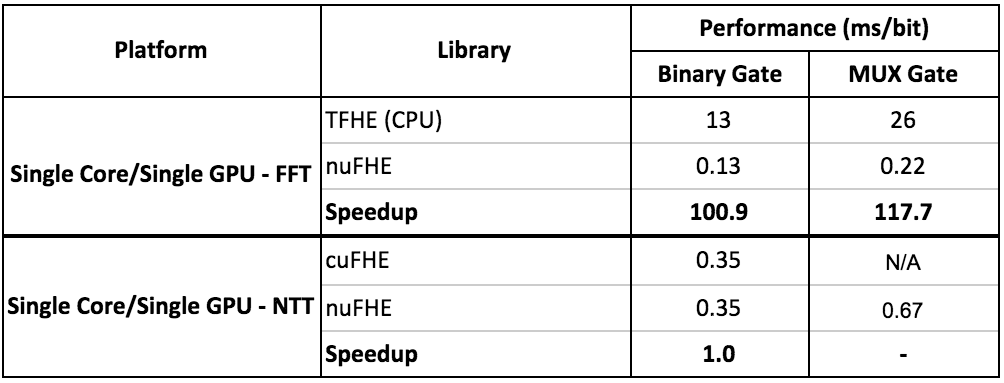
\includegraphics[width=10.5cm]{pdf/nufhe-benchmarks.pdf}
           \end{figure}
       \end{itemize}
    \end{frame}

    \begin{frame}
        \frametitle{Activities + done}
        \begin{itemize}
            \item Threshold m-of-n proxy re-encryption Umbral: done;
            \item Staking smart contracts: done;
            \item On-chain smart contract verification: done;
            \item On-chain enforcement of correctness: to do;
            \item NuCypher network: federated done, decentralized on the way;
            \item On-chain conditions for NuCypher network: to do after testnet;
            \item Research on FHE.
        \end{itemize}
    \end{frame}

    \begin{frame}
        \frametitle{Useful links}
        \begin{figure}
            \centering
            
\includegraphics[width=3cm]{pdf/nucypher_logo.pdf}
        \end{figure}
        Website: \url{https://nucypher.com}

        NuCypher network: \url{https://github.com/nucypher/nucypher/}

        PyUmbral: \url{https://github.com/nucypher/pyUmbral/}

        GoUmbral: \url{https://github.com/nucypher/goUmbral/}

        FHE: \url{https://github.com/nucypher/nufhe/}

        Discord: \url{https://discord.gg/7rmXa3S}

        Whitepaper: \url{https://www.nucypher.com/whitepapers/english.pdf}

        E-mail: \url{hello@nucypher.com}
    \end{frame}

    \begin{frame}
        \frametitle{FHE demo: homomorphic smart contracts assembly}
        \begin{figure}
            \centering
            \includegraphics[height=5.5cm]{pdf/terminal.pdf}
        \end{figure}
        \url{https://github.com/nucypher/Sputnik/}
    \end{frame}

\end{document}

